% Kompiuterijos katedros ir kibernetinio saugumo laboratorijos šablonas
% Template of Department of Computer Science II or cybersecurity laboratory
% Versija 1.3 2021 m. birželis [ March, 2015]

\documentclass[a4paper,12pt,fleqn]{article}
\usepackage[unicode,colorlinks=false]{hyperref}


\usepackage[utf8x]{inputenc}
%

\usepackage[L7x]{fontenc}
\usepackage{times}
\usepackage{ucs}
\usepackage{microtype}
\DisableLigatures{encoding = *, family = *}
 %package to switch the language
\usepackage{etoolbox}

  %set up of the page margins
\usepackage[top=2cm, bottom=2cm, left=3cm, right=1.5cm]{geometry}

 %1.1 line spacing
\linespread{1.1}


  %page numbering at the right side
\usepackage{fancyhdr}
\pagestyle{fancyplain}
\fancyhf{}
\renewcommand{\headrulewidth}{0pt} 
\fancyhfoffset[RO]{0cm}

  %to number at the bottom (exchange lines to number at the top)
\rfoot{\thepage}
  %\rhead{\thepage} %

% \usepackage[usenames,dvipsnames]{pstricks}
\urlstyle{same}
\hypersetup{
%  citecolor=Blue,
%  linkcolor=Blue,
%  urlcolor=Blue
pdfborder={0 0 0 }
}

 %for includegraphics
\usepackage{graphicx}



\usepackage[toc,page]{appendix}


\usepackage{caption}

 %for source codes
\usepackage{listings}
\lstset{commentstyle=\color{red},xleftmargin=10pt, framexleftmargin=6pt, numbersep=1mm, frame=single, numbers=left,numberstyle=\footnotesize,extendedchars=\true, inputencoding=utf8x,basicstyle=\footnotesize,extendedchars=true,
 keywordstyle=\color{black}\bfseries, breaklines=true, breakautoindent=true,framesep=8pt,linewidth=0.95\textwidth
}

 %for algorithms
\usepackage{algorithm}
\usepackage{algorithmic}
 %instead of the above two packages we can use algorithms2e
 %\usepackage[boxed,linesnumbered,vlined,slide]{algorithm2e}

 %special symbols
\usepackage{amsfonts}
\usepackage{amssymb}
\usepackage{amsmath}

 %for theorem like environments
\usepackage{amsthm}

 \usepackage{datetime}
 \renewcommand{\dateseparator}{--}


% SI system units
\usepackage{siunitx}
\sisetup{detect-all}
% Problem with fonts \SI{x.xx}{\micro\metre}, solved with updmap-sys --enable Map=utm.map
\renewcommand{\sfdefault}{uhv}
\renewcommand{\rmdefault}{utm}
\renewcommand{\ttdefault}{ucr}

% List management (itemize, etc.)
\usepackage{enumitem}

\newcommand*{\urlw}[1]{\href{#1}%
            {\nolinkurl{#1}}}

\numberwithin{equation}{section}


%%%%%%%%%%% lino įdėta
%
\usepackage{pifont,mdframed}

\newenvironment{warning}
  {\par\begin{mdframed}[linewidth=2pt,linecolor=red]%
    \begin{list}{}{\leftmargin=1cm
                   \labelwidth=\leftmargin}\item[\Large\ding{43}]}
  {\end{list}\end{mdframed}\par}
  
\usepackage{url}
\usepackage{svg}
\usepackage{graphicx}

\newtoggle{inLithuanian}
 %If the report is in Lithuanian, it is set to true; otherwise, change to false
\settoggle{inLithuanian}{true}

%create file preface.tex for the preface text
%if preface is needed set to true
\newtoggle{needPreface}
\settoggle{needPreface}{false}

\newtoggle{signaturesOnTitlePage}
\settoggle{signaturesOnTitlePage}{true}


\theoremstyle{definition}
\newtheorem{definition}{\keyWordDefinition}
\newtheorem{example}{\keyWordExample}
\def\QED{\unskip\nobreak\hfill\kern5pt$\Box$}

\iftoggle{inLithuanian}{
%\usepackage[L7x]{fontenc}
\usepackage[english,lithuanian]{babel}

\newcommand{\todayiso}{\the\year \dateseparator \twodigit\month \dateseparator \twodigit\day}


\renewcommand{\today}{\number\year\space m. \space \ifcase\month\or
  sausio\or vasario\or kovo\or balandžio\or gegužės\or birželio\or
  liepos\or rugpjūčio\or rugsėjo\or spalio\or lapkričio\or
  gruodžio\fi
  \space\number\day\space d.}


 \usepackage{tocloft}
 \renewcommand\cftsecaftersnum{.} 
 \renewcommand\cftsubsecaftersnum{.} 
 \renewcommand\cftsubsubsecaftersnum{.}

 \usepackage{VUMIFKK}

 \DeclareCaptionLabelFormat{captionlt}{#2 #1}
   %smth is not fine with algorithms 
 \DeclareCaptionLabelFormat{captionltalg}{#2 #1 algoritmas}

 \usepackage{indentfirst}
 \renewcommand{\appendixtocname}{Priedai}
 \renewcommand{\appendixpagename}{Priedai}
 \renewcommand{\contentsname}{Turinys} 

 \renewcommand{\lstlistingname}{išeities kodas}
 \renewcommand{\figurename}{pav}
 \renewcommand{\tablename}{lentelė}


 \captionsetup*[lstlisting]{   
 labelsep=period,labelformat=captionlt
 }
 \captionsetup*[figure]{   
% labelsep=period,
 labelsep=space, %babel redefines pav to pav.
 labelformat=captionlt
 }
 \captionsetup*[table]{   
  labelsep=period,
  labelformat=captionlt
 }
 \renewcommand{\algorithmicrequire}{\textbf{Įvestis:}}
 \renewcommand{\algorithmicensure}{\textbf{Išvestis:}}

 \captionsetup*[algorithm]{   
 labelsep=period,labelformat=captionltalg
 }

\renewcommand{\thmhead}[3]{#2 #1#3}

}
{
%\usepackage[OT1,T1]{fontenc}
%\usepackage[L7x]{fontenc}



\usepackage[english]{babel}
\newcommand{\todayiso}{\twodigit\month \dateseparator \twodigit\day \dateseparator \the\year}
 \captionsetup*[algorithm]{   
 labelsep=period
 }
\captionsetup*[lstlisting]{   
 labelsep=period
 }
 \captionsetup*[figure]{   
 labelsep=period
 }
 \captionsetup*[table]{   
 labelsep=period
 }


}

%some kywords
 \def\keywordAbstract{\iftoggle{inLithuanian}{Santrauka}{Abstract}}
 \def\keywordAbstractOther{\iftoggle{inLithuanian}{Summary}{Santrauka}}
 \def\keyWordIntroduction{\iftoggle{inLithuanian}{Įvadas}{Introduction}}
 \def\keyWordConclusions{\iftoggle{inLithuanian}{Išvados ir rekomendacijos}{Conclusions and Recommendations}}

 \def\keyWordPreface{\iftoggle{inLithuanian}{Pratarmė}{Preface}}
 \def\keyWordAppendice{\iftoggle{inLithuanian}{Priedas}{Appendix}}
 \def\keyWordSignature{\iftoggle{inLithuanian}{parašas}{signature}}
 \def\keyWordDefinition{\iftoggle{inLithuanian}{apibrėžimas}{Definition}}
 \def\keyWordExample{\iftoggle{inLithuanian}{pavyzdys}{Example}}

\newcommand{\bothabstracts}[3]{
\setcounter{secnumdepth}{0}
\newpage
\hspace{2cm}
{\centering{\section{\keywordAbstract}}}

#1
\newpage
\hspace{2cm}
{\centering \section{\keywordAbstractOther}}

\begin{center}{\textbf{#2} }\end{center}

 #3
\setcounter{secnumdepth}{3}
}

 %non-numbered sections: #1 param: for labeling sec:#1, #2 -section title
\newcommand{\sectionWithoutNumber}[2]{\newpage
%\hspace{2cm}
\section*{#1}
\label{sec:#2}
\addcontentsline{toc}{section}{\nameref{sec:#2}}%{#3}
 }



\newcommand{\referenceSources}[1]{
\newpage
\cleardoublepage
\phantomsection
\iftoggle{inLithuanian}{
 \renewcommand{\refname}{Literatūros šaltiniai}

 \addcontentsline{toc}{section}{Literatūros šaltiniai}
 \markboth{\refname}{Literatūros šaltiniai}
 }
{

\addcontentsline{toc}{section}{References}
\markboth{References}{References}
}

\bibliographystyle{unsrt}
\bibliography{#1}
}



 \newcommand\authorsignature[1]{
\begin{flushright}
 \begin{minipage}[b]{0.45\textwidth}
  \centering
  \rule{\textwidth}{0.5pt}\\
   #1
  \end{minipage}
\end{flushright}
 }




 \newcommand\authorsignatures[5]{%
   \vspace{1cm}
   \authorsignature{#1}
   \ifstrequal{#2}{}{}{\vspace{0.3cm}
     \authorsignature{#2}
     \ifstrequal{#3}{}{}{\vspace{0.3cm}
      \authorsignature{#3}
      \ifstrequal{#4}{}{}{\vspace{0.3cm}
        \authorsignature{#4}
        \ifstrequal{#5}{}{}{\vspace{0.3cm}
         \authorsignature{#5}       
        }
      }
    }
} 
}

\newcommand{\authortitle}{
\iftoggle{signaturesOnTitlePage}{
\tiny{\keyWordSignature}
}{}
}

\newcommand{\depttitlepage}[8]
{
\thispagestyle{empty}
\begin{center}


\includegraphics[width=2cm]{jb_VU_zenklas}

%\vspace{-1cm}

\iftoggle{inLithuanian}
{ 
  VILNIAUS UNIVERSITETAS\\
  MATEMATIKOS IR INFORMATIKOS FAKULTETAS\\
  INFORMATIKOS INSTITUTAS\\
  KOMPIUTERIO IR DUOMENŲ MODELIAVIMO KATEDRA
}
{
  VILNIUS UNIVERSITY \\
  FACULTY OF MATHEMATICS AND INFORMATICS \\
  INSTITUTE OF COMPUTER SCIENCE\\
  <<DEPARTMENT OF COMPUTATIONAL AND DATA MODELING>> OR \\ <<CYBERSECURITY LABORATORY>>
}

\vspace{5cm}

#1\\
\vspace{0.5cm}
\textbf{\Large #2}
\end{center}

\vspace{5cm}


\hspace{0.5\textwidth}
\begin{minipage}{0.4\textwidth}
 \begin{flushleft} 
\iftoggle{inLithuanian}
{
 \ifstrequal{#3}{}{}{Atliko:\\[5pt]}
}
{
\ifstrequal{#3}{}{}{Done by:\\[5pt]}
}
%\noindent
\begin{tabular}{@{}lr}%\setlength\tabcolsep{0pt}
\ifstrequal{#3}{}{}{#3&\hspace{2cm}\authortitle\\[5pt]}
\ifstrequal{#4}{}{}{#4&\authortitle\\[5pt]}
\ifstrequal{#5}{}{}{#5&\authortitle\\[5pt]}
\ifstrequal{#6}{}{}{#6&\authortitle\\[5pt]}
\ifstrequal{#7}{}{}{#7&\authortitle\\}
\end{tabular}

\end{flushleft}

\end{minipage}

\vspace{0.5cm}
\hspace{0.5\textwidth}
\begin{minipage}{0.4\textwidth}
 \begin{flushleft} 

\ifstrequal{#8}{}{}
{

\iftoggle{inLithuanian}
{
Vadovas:
}
{
Supervisor:
}

#8

}

\end{flushleft}

\end{minipage}


\vfill

\begin{center}
Vilnius\\
\the\year
\end{center}

\iftoggle{needPreface}{
 \sectionWithoutNumber{\keyWordPreface}{preface}
Pratarmės (Preface) informacija


\iftoggle{inLithuanian}
{
\vspace{\baselineskip}\hfill
\today
}
{
 \vspace{\baselineskip}\hfill \today
}

 \vspace{5cm}

\iftoggle{signaturesOnTitlePage}{}
{
\authorsignatures{#3}{#4}{#5}{#6}{#7}
}
}{}
\newpage
}


\begin{document}
 % #1 -report type, #2 - title, #3-7 students, #8 - supervisor
 \depttitlepage{IV semestro projektinis darbas}{Diskų kopijų teisminė ekspertizės Android įrenginiuose tyrimas\\{\small Disk image forensics research in Android devices}}{Matas Niewulis} 
 {}{}{}{}% students 2-5
 {Lekt. Virgilijus Krinickij}

\tableofcontents

%keywords and notations if needed
\sectionWithoutNumber{Sutartinis terminų žodynas}{keywords}

 \begin{itemize}
     \item \textbf{„ADB“} – „Android Debug Bridge“ – „Android“ diagnostikos tiltas, skirtas komunikuoti su „Android“ įrenginiais per komandinę eilutę ir vykdyti įvairius veiksmus, pvz., diegti programinę įrangą, siųsti komandas ir peržiūrėti įrenginio informaciją. Tai yra sujungimas tarp mobiliojo įrenginio ir kompiuterio
     \item \textbf{„Bash“} – Unix tipo operacinės sistemos komandinės eilutės interpretatorius, naudojamas vykdyti komandų rinkinius, automatizuoti užduotis ir kurti skriptus. Tai populiari komandinės eilutės programa, dažnai naudojama „Linux“ aplinkoje.
     \item \textbf{„Boot“} – Įrenginio ar kompiuterio operacinės sistemos ar programinės įrangos užkrovimo procesas, kuris vykdomas įjungus įrenginį. Tai pirmasis žingsnis paleidžiant įrenginį kuris užtikrina, kad operacinė sistema ar programa būtų įkrauta ir veiktų tinkamai.
     \item \textbf{CWD} - Current Working directory - esamasis darbo katalogas
     \item \textbf{„Device driver“} – įrenginio tvarkyklė – Programinės įrangos komponentas, kuris leidžia operacinės sistemai sąveikauti su konkrečiu įrenginiu. Įrenginio tvarkyklės užtikrina, kad įrenginys būtų tinkamai valdomas ir galėtų veikti su kitomis sistemomis.
     \item \textbf{Flashing (įrašymas)} - Šis terminas apibūdina procesą, kai įrenginio atmintyje esantis programinis įrašas (pavyzdžiui, Android operacinė sistema) yra pakeičiamas kitu programiniu įrašu (pavyzdžiui, „custom ROM“), naudojant specialų programinį įrankį. Tai gali būti naudinga tiems, kurie nori atnaujinti savo Android įrenginio operacinę sistemą, arba nori pasiekti papildomas funkcijas, kurių nėra standartinėje sistemoje. Įrašyti galime taip pat particijų atvaizdus, pvz. TWRP atvaizdą.
     \item \textbf{„Loop device“}- Virtualus įrenginys, kuris leidžia naudoti failą ar atminties sritį kaip blokinį įrenginį. Yra naudingas, kai reikia sukurti virtualų įrenginį, kuris veiktų kaip realus blokinis įrenginys, pavyzdžiui disko atvaizdas.
     \item \textbf{Particija} – Fizinis arba loginis laikmenos skyrius, skaidinys, kuris yra paskirstytas išmaniuose telefonuose ar kituose įrenginiuose. Particijos leidžia atskirti ir organizuoti skirtingus duomenų segmentus.
     \item \textbf{Particijos atvaizdas} – Particijos bitinė kopija (*.img failas).
     \item \textbf{„Root“}  - Administratoriaus prieigos teisių aukščiausias lygis „Android“ operacinėje sistemoje. Šis lygis suteikia galimybę vykdyti privilegijuotas operacijas, pakeisti sistemą sudarančius failus ir valdyti įrenginį plačiau.
     \item \textbf{„Shell script“} – Eilutės komandų rinkinys, kuriuo gali būti automatizuojami įvairūs veiksmai. Skriptas yra parašytas „Shell“ (arba „Bash“) kalba ir leidžia komandas per komandinės eilutės interpretatorių (*.sh failas)
     \item \textbf{Skriptas} - Programavimo kalbos tekstas, kuriame yra įrašytos instrukcijos ar komandos, skirtos vykdyti tam tikrus veiksmus. Skriptai yra naudojami automatizuoti procesus ir palengvinti tam tikras užduotis, pavyzdžiui, duomenų išgavimą iš įrenginio arba atlikti operacijas su failais.
     

 \end{itemize}

 %both abstracts
\bothabstracts{Išmanieji telefonai tapo vienu iš dažniausiai naudojamų komunikacijos priemonių dėl jų geriausio ryšio, funkcionalumo ir produktyvumo. Nuolat tobulėjant išmaniųjų telefonų technologijoms, atsiranda naujų lygių pavojai. Didžioji rinkos dalis pasitiki „Android“ operacinės sistemos telefonais, kuri yra svarbi jėga konkurencinėje rinkoje, „Android“ ir „iOS“ duopolyje. „Android“ telefonai kaupia milžinišką duomenų kiekį, kurį galima saugoti tiek vietiniu, tiek nuotoliniu būdu, todėl teismo ekspertams jie suteikia patikimų duomenų, kurie yra labai svarbūs teismo ekspertizei. \\

Šiame darbe siekiama sukurti dinamišką įrankį, skirtą duomenų išgavimui, analizei ir parengimui teismo ekspertizei. Įrankis sukurtas atsižvelgiant į tai, jog dauguma esamų įrankių nėra suderinami su visais „Android“ mobiliaisiais įrenginiais. Įrankio programavimui buvo naudojama „Shell Script“ kalbą. Visos komandas buvo automatizuotis ir suskirstytos į skirtingus skriptus, kurie palengvina teismo ekspertizės analizę. Šis įrankis gali būti  paleistais „Linux“ ar „Windows“ (su „Windows Subsystem for Linux“) operacinėse sistemose. Norint išgauti duomenis, naudojama „ADB Shell“ komunikacija, naudojant root lygį, kuris pasiekiamas paleidus neoficialų atstatymo režimą. Tyrimo metu buvo atsižvelgta į skambučių žurnalo istoriją, SMS žinutes, naršyklės istoriją, nuotraukas ir kitus failus, kurie yra svarbūs teismo ekspertizei. Norint palengvinti tolimesnę duomenų analizę, jie yra suskirstomi į aplankus. \\

Darbo eigoje sukurta priemonė išgauna įrenginio duomenų particijos atvaizdą, jį išsaugo ir tinkamai suformatuoja išgautus duomenis taip, kad būtų patogu juos naudoti bylų sprendimui. Sukurtas įrankis veikia su dauguma „Samsung“ įrenginių, kurie neturi įjungto priverstinio šifravimo (angl. force encrypt) funkcijos. Jis taip pat gali būti pritaikytas duomenų ištraukimui iš kitų gamintojų įrenginių.}%tex-file of abstract in original language
{Disk image forensics research in Android devices} %if work is in LT this title should be in English
{Smartphones have become one of the most commonly used communication devices due to their improved connectivity, functionality, and productivity. As smart technologies continue to advance, new levels of potential risks emerge. The majority of the market relies on Android operating system phones, which holds a significant position in the competitive market, forming an Android-iOS duopoly. Android devices store a vast amount of data, which can be stored locally or remotely, providing forensic experts with reliable data that is crucial for forensic investigations.\\

The objective of this coursework is to develop a dynamic tool for data extraction, analysis, and preparation for forensic examination. The tool has been developed considering the fact that most existing tools are not compatible with all Android mobile devices. The tool has been programmed using the Shell Script language, utilizing commands that have been automated and divided into separate scripts, which facilitate forensic analysis. This tool can be used on Linux or Windows (with Windows Subsystem for Linux) operating systems. To access the data, ADB Shell communication is utilized on the root level, which can be achieved by booting into an unofficial recovery mode. During the development, considerations have been made for call log history, SMS messages, browser history, photos, and other files that are relevant to forensic examination. Data is organized into directories to facilitate further analysis.\\

The developed tool extracts the data partition image of the device, saves it, and properly formats the extracted data for convenient use in case resolution. This tool works with most Samsung devices that do not have the force encrypt feature enabled, and it can also be adapted for devices from other manufacturers.\\}%tex-file of abstract in other language

 %Introduction section: label is sec:intro
\sectionWithoutNumber{\keyWordIntroduction}{intro}
\textbf{Darbo aktualumas} Mobilieji telefonai per pastaruosius metus tapo populiarūs dėl savo didelio funkcionalumo, prieinamumo ir produktyvumo. Tačiau šios pažangios technologijos taip pat atnešė naujų iššūkių ir pavojų, ypač kriminalistikoje. Kriminalistinėje veikloje mobilieji įrenginiai tapo duomenų kaupimo ir komunikacijos priemonėmis, o juose sukaupti duomenys tapo svarbia medžiaga teisminėse ekspertizėse.\\

\textbf{Darbo problema} Duomenų tyrimai rankiniu būdu užima daug laiko bei yra mažiau tikslūs ir saugūs, nes daugumą procedūrų norint išgauti duomenis yra pasikartojančios ir galėtų būti automatizuotos naudojant skriptus, kurie automatiškai išgautų duomenis iš atvaizdo. Be to, pats atvaizdo sukūrimas sudaro galimybes efektyvesnei analizei, nes keli darbuotojai gali dirbti su tuo pačiu atvaizdu, pasidalinti darbais. Deja, dėl žymių skirtumų tarp skirtingų mobiliųjų telefonų modelių bei operacinės sistemos variacijų, labai sunku sukurti įrankį, kuris automatiškai tiktų kiekvienam telefonui, be jokių modifikacijų.
„Android“ operacinėje sistemoje su kiekvienu atnaujinimu, duomenų pasiekimo kelias gali būti ribojamas. Mobilieji telefonai su „Android“ operacine sistema vis dažniau vartojami, todėl dažnai tenka daryti jų teisminę ekspertizę. Sukurtas įrankis palengvintų darbuotojams duomenų išgavimo procesą. \\

\textbf{Darbo objektas.}  Prijungus telefoną, sukūrus jo disko atvaizdą, sumontavus (angl. mounted) jį bei išgavus ir apdorojus duomenis, tyrėjas galėtų atlikti daug kokybiškesnį bei greitesnį darbą, naudojant automatizuotą įrankį. Įrankio veikimo principas paprastas - kompiuteryje įrašytas įrankis prisijungia prie telefono, ištraukia atminties atvaizdą, pasiekia jame esančią informaciją, tvarkingai ją suformatuoja ir paruošia tolimesniam tyrimui. Įrankis turėtų  išgauti duomenis vientisa tvarką, nes bet koks vientisumo pažeidimas sunaikintų duomenų integralumą.\\

\textbf{Darbo tikslas.}  Darbo tikslas yra sukurti automatizuotą įrankį, kuris ištirtų „Android“ įrenginį ir palengvintų jo tyrimo procesą. Šis darbas aprašo, kaip galima atlikti mobilių telefonų, veikiančių su „Android“ operacine sistema, teisminę ekspertizę.\\

\textbf{Darbo uždaviniai: }
\begin{itemize}
 \setlength{\itemsep}{1pt}
  \setlength{\parskip}{0pt}
  \setlength{\parsep}{0pt}
    \item  Apžvelgti Android įrenginio architektūrą
    \item  Pademonstruoti veikimo modelį
    \item  Apžvelgti sukurto įrankio funkcionalumą
    \item  Aprašyti ateities planus tyrimui
\end{itemize}


 %the main part
 \newpage
\section{Susijusių darbų analizė}
Sparčiai besivystančioms informacinėms technologijoms reikalingi metodai skirti atlikti  efektyvią kompiuterinių ar mobiliųjų diskų ekspertizę. Šioje srityje yra sukurti keli programinės įrangos įrankiai, tačiau dauguma jų yra mokami, komerciniai ar uždaro kodo. Negalime naršyti šių įrankių šaltinio kodų ir giliau nagrinėti jų veikimo principo. \\


„Android“ įrenginių ekspertizėms sunku sukurti universalų programinį įrankį, nes „Android“ įrenginiai skiriasi savo architektūromis, duomenų kaupimo būdu ar operacinės sistemos versijomis (pvz. 9,10,11...) ir variantais (pvz. MIUI, Samsung OneUI, Huawei EMUI...). Skirtumai sutinkami taip pat sistemos saugumo lygiuose, failų struktūrose.  Remiantis kitų mokslinių tyrėjų darbų išvadomis, galime teigti jog universalus ir automatizuotas įrankis dar nesukurtas \cite{practicalforensics} \cite{AutomatedForensics}\\


Net jau ir sukurti įrankiai, po ,„Android“ įrenginio sistemos atnaujinimo, gali nustoti veikti. 
Kadangi įrenginiai yra dažniausiai naujinami per 2-3 metus gamintojo teikiamais saugumo naujiniais. Gali iškilti atvejis, kai įrenginys veikiantis su 2023m gegužės naujiniu bus sėkmingai panaudotas su įrankiais, o toks pats įrenginys su 2023m. birželio naujiniu jau nesuveiks. Policija ir kitos valstybės saugumo institucijos turi sukurtus tam tikrus įrankius, tačiau jie plačiai visuomenei nėra prieinami. Greičiausiai naudojamos CVE ar „zero-day“ spragos, kurios suteikia galimybe pasiekti duomenis daugumoje įrenginiu. Dėja tai reikalauja žinių bei skirti daug laiko kiekvienam atvejui.\\


Tokių problemų nėra kompiuterių srityje. Galima teigti jog visi kompiuteriai, kuriuos naudojame, veikia su viena iš trijų pagrindinių operacinių sistemų: „Windows“, „Linux“ bei „MacOS“. Šios operacinės sistemos duomenis užrašo į atskirą diską (mechaninį HDD ar puslaidininkinį SSD), kurį galime atskirai atjungti nuo įrenginio ir analizuoti jį su daugeliu pažengusių įrankių leidži. Tokie įrankiai leidžia išgauti ištrintus failus, praleisti slaptažodžius ar lengvai sukurti bitines disko kopijas. Remiantis „Windows Surface RT tablet forensics“ moksliniu darbu, galime teikgti jog „Windows“ įrenginiams yra sukurta daug ekspertizių metodų. \cite{SurfaceRTForensics}
Sukurtų įrankių yra daug, bet deja jie veikia tik su kompiuteriais, o ne mobiliais įrenginiais. Kompiuterių tyrimo atvejams yra sukurta metodika bei programinė įranga, kuria sekant galime lengvai atlikti tyrimą. „Android“ įrenginiams tokia metodika dar nėra sukurta\\

\newpage
\section{Android įrengino architektūra}
Šiame skyriuje apžvelgiami operacinės sistemos veikimo principai bei versijos, kurios yra esminė informacija reikalinga sėkmingam duomenų
\subsection{Operacinės sistemos architektūra}
Įrenginiai su „Android“ operacine sistema, skiriasi nuo tradicinių kompiuterių. Architektūrų skirtumai matomi tiek apatinėje įrangoje (angl. hardware) tiek skirtingose operacinėse sistemose. „Android“, kaip ir „Linux“, priklauso tai pačiai „UNIX“ operacinių sistemų šeimai, tačiau ji žymiai skiriasi nuo tradicinės Linux aplinkos.\cite{AndroidLinuxDifferences}

Mobiliųjų telefonų ekspertizės atveju, duomenų išgavimo procesas žymiai skiriasi nuo kompiuterių diskų analizės. \cite{forensicsPCvsPHONE} Analizuojant nešifruotus Linux ar Windows kompiuterių diskus, galima juos gan lengvai prijungti prie kito kompiuterio ir išgauti juose esančius duomenis. „Android“ įrenginiuose duomenų išgavimo procesas gali būti žymiai sudėtingesnis, dėl skirtingų operacinės sistemos versijų, bei saugumo ar paleidimo įkroviklio (angl. bootloader),  kuris yra atsakingas už įrenginio operacinės sistemos paleidimą, variacijų \cite{bootloaderdiff}.

\subsection{Versijos}
„Android“ įrenginiuose, svarbu atkreipti dėmesį į operacinės sistemos versiją, nes priklausomai nuo jos, duomenų pasiekimas gali būti apsunkintas ar neįmanomas.
„Android“ operacinės sistemos pirma versiją „1.0“ išleista 2008 m. \cite{AndroidFirstVersion} Šiais metais jau pasiekiama „13“ versija, ir sistema toliau tobulinama. Prieš pradedant darbą, svarbu patikrinti sistemos versiją.

Norint sėkmingai panaudoti ekspertizei sukurtą įrankį, būtina susijungti su telefonu ir jam suteikti „root“ teises. Alternatyviai galime paleisti jį neoficialiame atstatymo režime, (angl. „custom recovery“)., kuriame turime prieiga prie visos telefono atminties ir dirbame kaip „root“ vartotojas.

\section{Įrankio veikimas}

Žinant svarbiausius architektūros elementus, galime sukurti veikimo modelį (1 pav.):
\begin{figure} [h]
    \centering
    \includesvg[width=380pt]{chart1.svg}  
    \caption{UML veiklos diagrama}
    \label{fig:flowchart}
\end{figure}


Norint pradėti duomenų išgavimo procedūra, reikia paleisti „main“ skriptą, pasirinkti norima funkciją ir prijungti įrenginį prie kompiuterio naudojant USB laidą. Paleidus įrankį, vykdomi veiksmai, atitinkamai nuo pasirinktos įrankio funkcijos: disko atvaizdo automatinis išgavimas, disko atvaizdo rankinis išgavimas, duomenų išgavimas iš disko atvaizdo, išgautų duomenų bazių išvedimas į skaitoma .txt failą ar atvaizdo išgavimas TWRP rėžime. Atvaizdas kopijuojamas į kompiuterį. Atvaizdas montuojamas, ir iš jo išgaunami duomenys. Išgautos duomenų bazės yra analizuojamos, ir jų rezultatai, kartu su visais kitais reikiamais failais, pateikiami viename aplanke.


\section{Įranga bei jos paruošimas}

Tyrimo praktinėje dalyje naudojau du mobiliuosius įrenginius - „Samsung Galaxy S3 Neo“ („Android“ versija 4.4.2) ir „Samsung Galaxy S5“ („Android“ versija 6.0.1). Abu įrenginiai buvo sėkmingai panaudoti numatytiems praktinės dalies veiksmams. Testams buvo planuojama naudoti dar tris modelius: „Google Nexus 5“ („Android“ versiją 6.0.1), „Oneplus 2“ („Android“ versija 6.0.1) bei „Samsung Galaxy S20 FE“ („Android“ versija 13), tačiau jie neatitiko šiam įrankiui. „Google Nexus 5“ kaip ir „Oneplus 2“ neturi galimybės prijungti microSD kortelės, tad atvaizdo išgavimas būtų buvęs sunkus. Pagrindinė problema yra panaudotas paleidimo įkroviklis (angl. „bootloader“). Šie įrenginiai naudoja „fastboot“ paleidimo įkroviklį. Norint panaudoti „custom recovery“ metodą, reikėtų atrakinti paleidimo įkroviklį, tuo pačiu ištrinant visus duomenis. Įrenginiams buvo galimybė suteikti „root“ teises naudojant programėlę „KingRoot“, bet šiam procesui telefonas turi būti be ekrano užrakto. 

Programėle „Kingroot“ suteikianti „root“ teises vienu paspaudimu jau neveikia \cite{KingrootNoLongerWorks} . „Kingroot“ serveriai bei tinklalapis „www.kingroot.net“ neveikia, be to programėlė nėra pilnai saugi, nes jungiasi prie kiniškų serverių\cite{XDAKingroot}, bei naudoja saugumo CVE spragas, norint suteikti „root“ teises, todėl būtina naudoti alternatyvius metodus. \cite{kingroot}

„Samsung Galaxy S20 FE“ yra originaliai šifruojamas su „force encrypt“ funkcija. Šiai dienai, nėra galimybės išgauti duomenų iš šifruoto įrenginio, o net jeigu pavyktų duomenis išgauti, jų iššifravimas gali trukti ilgai, ar reikalauti superkompiuterio.

Dėl šių priežasčių darbą atlikau su „Samsung Galaxy S3 NEO“ įrenginiu. Jis neatitiko „KingRoot“ reikalavimų, todėl įrenginiui sukūriau skriptą, kuris įrašo neoficialų „TWRP“ (Team Win Recovery Project)  \cite{twrp} atstatymo režimą. Dirbant atstatymo rėžime, galime išgauti duomenis iš įrenginio net ir su ekrano užraktu. Duomenų išgavimas su ekrano užraktu reikalauja rankiniu būdu įvesti įrenginį į „Download mode“ įrašymo būseną.

Atvaizdo sukūrimui reikalinga microSD kortelė kurios talpa didesne negu vidinės telefono atminties talpa. Yra galimybė atvaizdą gauti naudojant TCP/IP sujungimą, jeigu dirbame su root teisėmis operacinėje sistemoje. Deja, atstatymo režime nėra galimybės prijungti prie tinklo.

Įrenginio analizei reikalingas kompiuteris. Duomenų ištraukimas gali vykti „Windows“ bei „Linux“ operacinėse sistemose. Rekomenduojama naudoti Linux, bet įrankis gali būti panaudotas ir Windows operacinėse sistemose, su „Windows Subsystem for Linux“ \cite{WSL}, kuriame yra galimybė įdiegti reikiamus įrankius bei paleisti „Bash“ skriptą. Tokiu atveju reikia papildomai įdiegti reikiamas tvarkykles (angl. device driver)

Norint įrašyti į įrenginį neoficialų atstatymo režimą ir jį paleisti, galime naudoti atviro kodo „Heimdall“ įrankį \cite{heimdall}.  Naudojamas taip pat „ADB“ (angl. „Android Debug Bridge“) įrankis, kuris leidžia sujungti kompiuterį su mobiliu įrenginiu. Duomenų analizei reikalingas „sqlite3“ paketas, kuris padės apdoroti duomenis iš atvaizde esančių duomenų bazių.

\section{Įrankio paleidimas bei duomenų išgavimas}

Priklausomai nuo pasirinkto metodo, norint išgauti duomenis automatiniu būdu arba patikrinti „force-encrypt“ būseną, būtina įrenginyje įjungti USB derinimą (angl. „USB Debugging“). Tai galime padaryti menu „Kūrėjų parinktys“ (angl. Developer options) (2 pav.):

\begin{figure} [h]
    \centering
    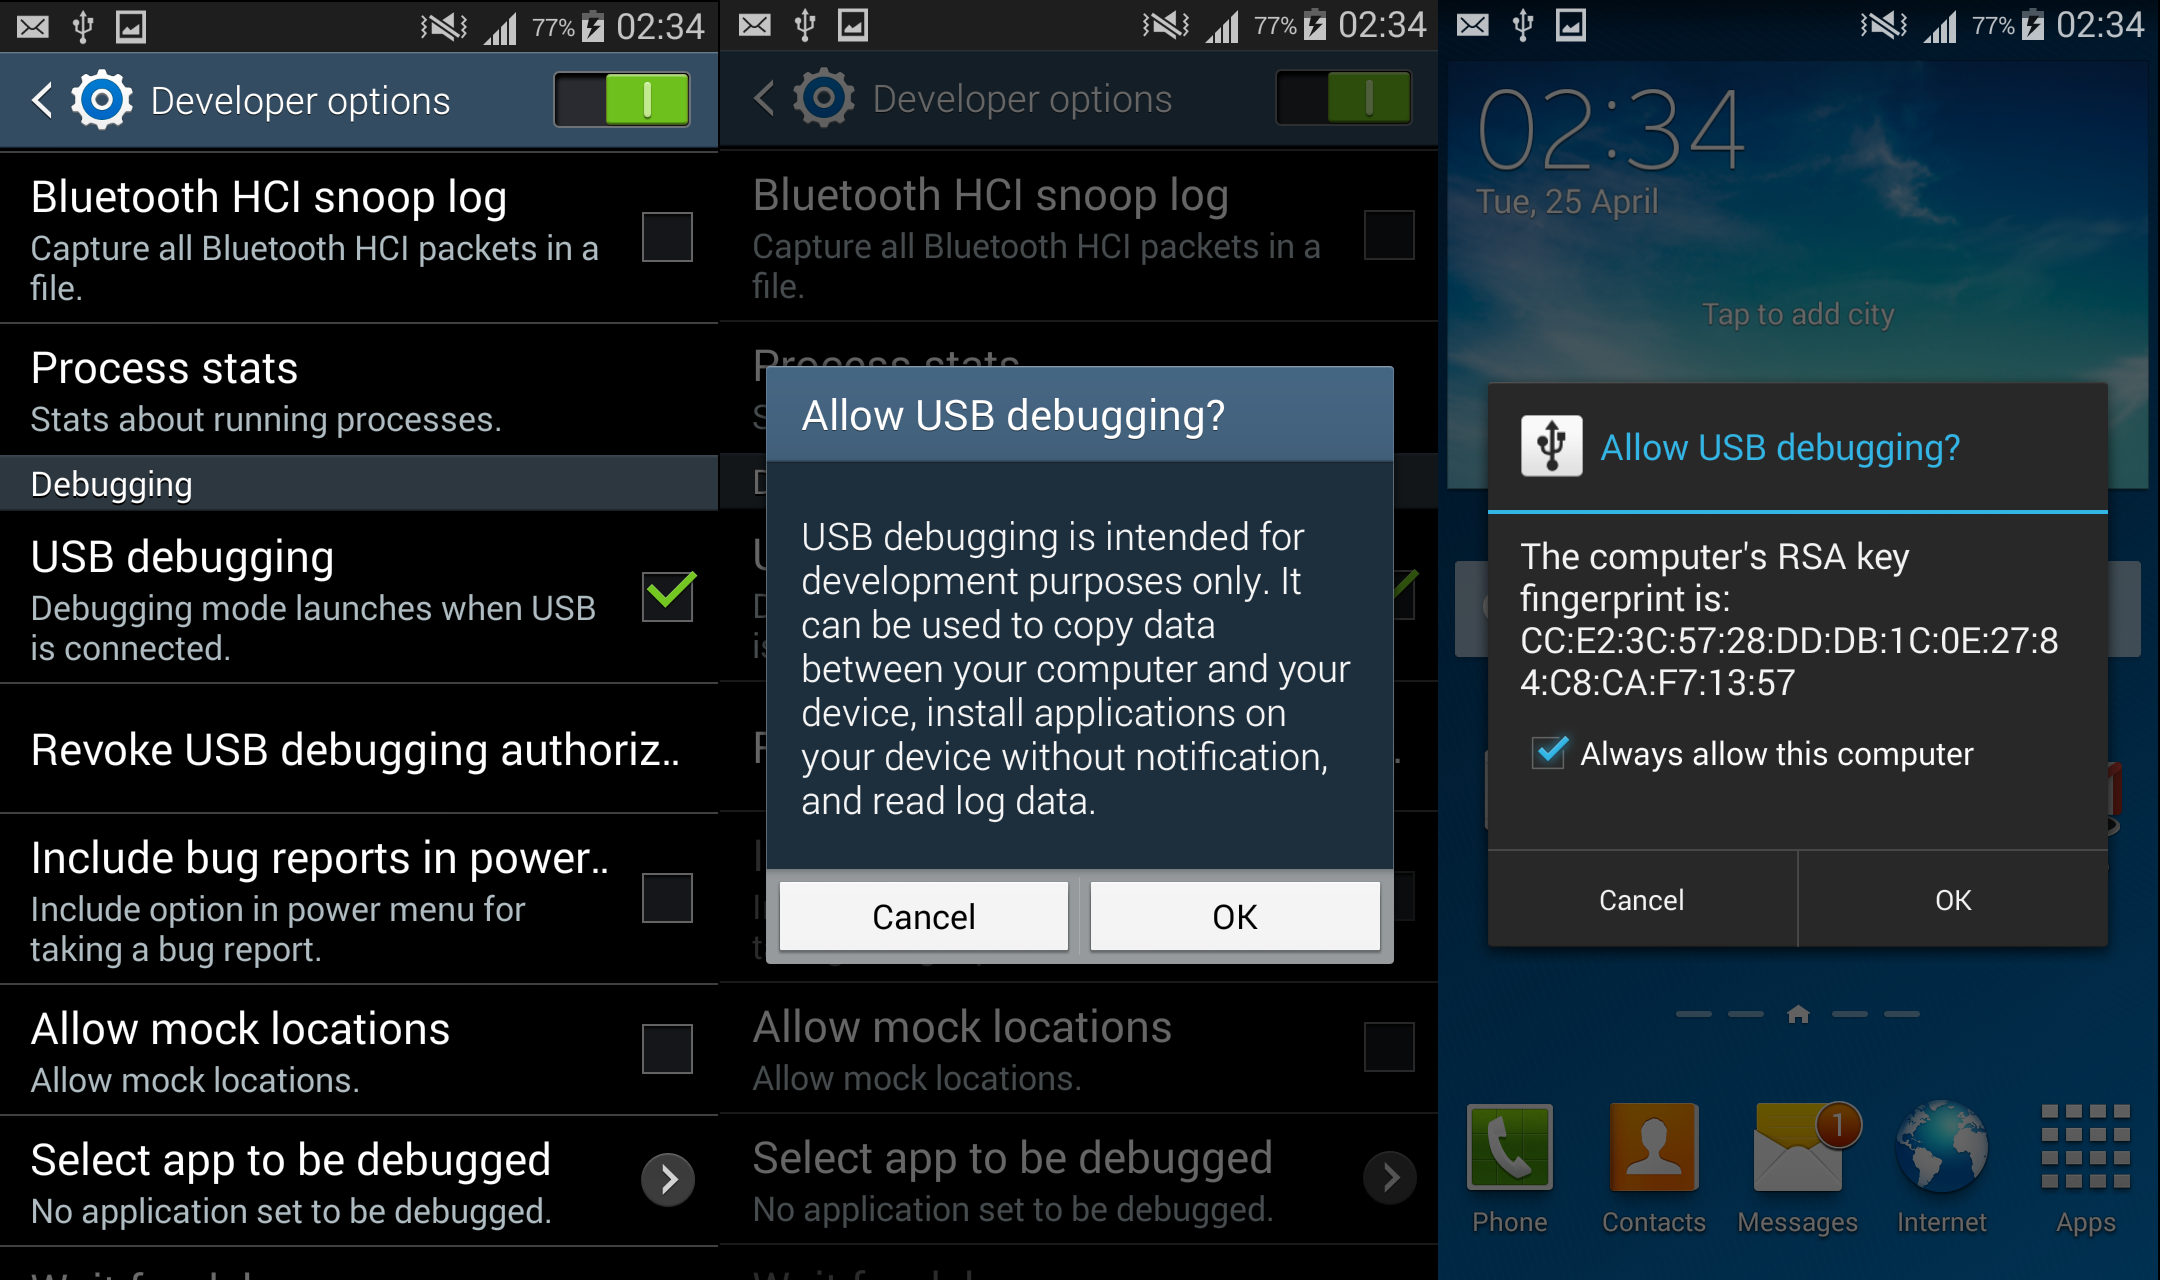
\includegraphics[width=0.85\textwidth]{usb-debugging.png}
    \caption{USB derinimas}
    \label{fig:debugging}
\end{figure}
Esant įrankio darbo aplanke, atveriame konsolės langą ir su komandą „./main.sh“ paleidžiame pagrindinį skriptą (skriptas paleidžia vieną iš devynių galimų skriptų esančių „bash“ aplanke). 
Kad įrankis sklandžiai veiktų, leidžiamam skriptui reikia suteikti aukštesnes teises.  Tam naudojame „sudo“  komandą. „Sudo“  yra Linux operacinės sistemos komanda, kuri leidžia vartotojams vykdyti komandas su aukščiausiomis „root“ teisėmis . Tai reiškia, kad naudotojas gali turėti aukštesnį leidimų lygį ir atlikti  daugiau operacijų. Veikimo principas panašus kaip administratoriaus teisės „Windows“ operacinėje sistemoje.\\

Paleidus ./main skriptą, su „sudo“ teisėmis, pasirodys menu su daugeliu parinkčių (3 pav.):

\begin{figure} [h]
    \centering
    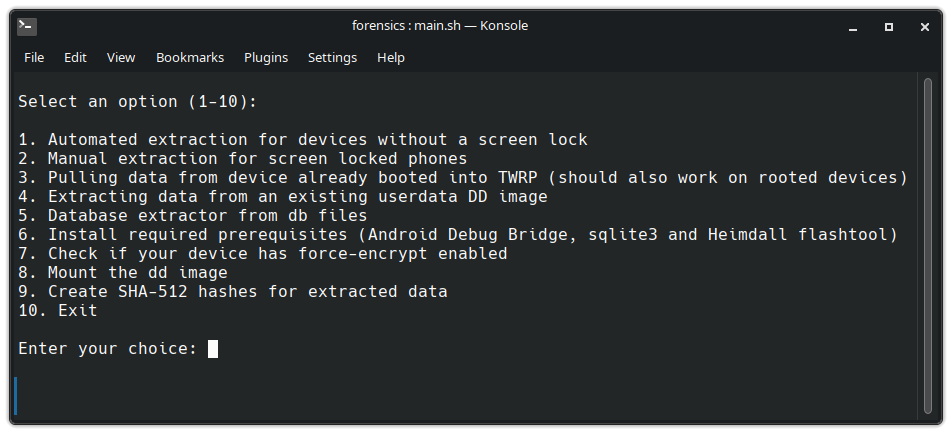
\includegraphics[width=0.85\textwidth]{terminal.png}
    \caption{Įrankio pagrindinis menu}
    \label{fig:terminal}
\end{figure}


\subsection{Įrankio atvaizdo gavimas automatiniu (1) atveju}    
\begin{enumerate}
    \item Paleidus skriptą suteikiame „sudo“ teises.
    \item Pirmą kartą paleidus įrankį, būtina įdiegti reikiamas bibliotekas bei programas - „ADB“, „heimdall-flash“ bei „sqlite3“. Pasirenkame parinktį, bei naudojamą operacinę sistemą. Kai įrankiai įsidiegs, paspaudus bent kokį klavišą grįžtame į pagrindinį menu.
    \item Parenkame pirmąjį skriptą, kuris skirtas automatiniam duomenų išgavimui.
    \item Skriptas sukuria „extracted\textunderscore data“ bei „mounted\textunderscore dd“ aplankus. Pirmasis skirtas išgautų duomenų bei rezultatų saugojimui, o antrasis naudojamas kaip montavimo katalogas (angl. „mount point“) įrenginio disko atvaizdui.
    \item Skriptas patikrins ar įrenginys prijungtas su USB derinimo režimu. Paprašys jį įjungti bei patvirtinti.
    \item  Paspaudus klavišą, įrankis įrašys (angl. flash) neoficialų atstatymo režimo atvaizdą. Šiam tikslui naudojamas atviro kodo įrankis „heimdall“, skirtas daugumai telefonų įrašinėti (angl. flash).
    \item Įrankis reikalaus fiziškai nuspausti reikiamus mygtukus, kad mobilų įrenginį įvesti į atstatymo režimą.
    \item  Skriptas patikrins ar įrenginys atitinkamai atskaitomas „ADB“ aplinkoje.
    \item Jeigu taip įvyks, įrankis išspausdins particijų lentelę, kurioje vartotojas turės įrašyti atitinkamą particijos pavadinimą, kurios etiketė „userdata“. Pavadinimas įrašomas mmcblk0pXX formatu rankiniu būdu, tam kad skriptą būtų galima pritaikyti kitiems mobiliems įrenginiams o ne tik šiam konkrečiam modeliui.
    \item Parinkus particiją, įrankis reikalaus suformatuoti ankščiau užmontuotą microSD atminties kortelę į „exFAT“ arba „EXT4“ failų sistemą. Formatavimas būtinas, nes dauguma kortelių būna suformatuotos „FAT32“ failų sistema, kuri neleidžia sukurti didesnio nei 4GB failo.
    \item Įrankis pradeda kurti bitinį „userdata“ particijos atvaizdą. 
    \item Naudojant „adb pull“ komandą, skriptas nukopijuoja atvaizdą į kompiuterio darbo aplanką.
    \item Kai atvaizdas jau nukopijuotas, visi duomenys esantys įrenginyje yra išsaugoti kompiuteryje.  
    \item Įrankis gražina originalų „recovery“ atvaizdą, kad įrenginys išliktų originalioje būsenoje.
    \item Įrankis užmontuoja „userdata“ particiją ir iš jos ištraukia duomenis. 
    \item Paspaudus bet kokį klavišą, grįžtama į pagrindinį menu.
    \item Iš pagrindinio menu reikia pasirinkti duomenų bazių ekstrakcijos funkciją, kad „extracted\textunderscore db“ aplanke susikurtų tekstiniai failai su reikiamais duomenimis.
    \item Pasirinkus „Exit“ funkciją, įrankis užbaigia darbą. Visi duomenys tvarkingai apdoroti teisminei analizei yra sukaupti „extracted\textunderscore data“ aplanke.
\end{enumerate}


\subsection{Įrenginio atvaizdo gavimas rankiniu (2) atveju}

Norint išgauti duomenis iš įrenginio, kuris užrakintas/apsaugotas ekrano užraktu, būtina naudoti antrą skriptą. 

Skripto veikimui nebūtinas USB derinimas, bet būtina rankiniu būdu įvesti įrenginį i „Download mode“ įrašymo (angl. flashing) režimą. Spaudžiame ir prilaikome „volume down + home + power“ klavišus, ir patvirtiname „volume up“ klavišu.

Veliau, visi veiksmai vyksta kaip aukščiau, nuo 5.1.6-5.1.13 bei 5.1.15-5.1.18

\subsection{Įrenginio atvaizdo gavimas iš įrenginio jau paleisto „TWRP“ režime (3) atveju}

Naudojant kito gamintojo ar modelio įrenginį, kuriame jau radome būdą kaip įrašyti ir paleisti „TWRP“ atstatymo režimą, galime naudoti šią parinktį. Veliau, visi veiksmai vyksta kaip aukščiau, nuo 5.1.8-5.1.13 bei 5.1.15-5.1.18

\subsection{Duomenų išgavimas iš jau turimo userdata.img dd atvaizdo (4) atveju}

Jeigu turime jau egzistuojantį įrenginio „dd“ atvaizdą, galime jį apdoroti. Pasirinkus šią funkciją, nurodome atvaizdo vietą (angl. path). Įrankis užmontuoja atvaizdą, bei išgauna iš jo reikiamus duomenis ir išsaugoja juos „extracted\textunderscore data“ aplanke.  Iš pagrindinio menu reikia pasirinkti duomenų bazių ekstrakcijos funkciją, kad „extracted\textunderscore db“ aplanke susikurtų tekstiniai failai su reikiamais duomenimis. Pasirinkus „Exit“ funkciją, įrankis užbaigia darbą

\subsection{Duomenų bazių analizė ir duomenų išvedimas į skaitomus .txt failus (5) atveju}

Pasirinkus šią funkciją, įrankis apdoroja .db failus, esančius extracted\textunderscore data aplanke. Skriptas gali analizuoti:
\begin{itemize}
 \setlength{\itemsep}{1pt}
  \setlength{\parskip}{0pt}
  \setlength{\parsep}{0pt}
    \item  SMS/MMS duomenų bazes
    \item  Kontaktų duomenų bazes
    \item  Skambučių registro duomenų bazes
    \item  Kalendoriaus įvykių duomenų bazes
    \item  Naršyklės duomenų bazes
    \item  Elektroninio pašto (e-Mail) duomenų bazes
\end{itemize}
Skriptas naudoja sqlite3 paketą, kad apdoroti duomenų bazes su SQL užklausomis. Po apdorojimo, rezultatai išvedami į tekstinius failus tokius kaip: messages.txt, contacts.txt, calendar.txt, login\textunderscore data.txt, cookies\textunderscore data.txt, call\textunderscore logs.txt, browsing\textunderscore history.txt.

Įrankis gali taip pat išgauti užrašytus naršyklėje slaptažodžius, kartu su prisijungimo vardu ir prisijungimo tinklalapio adresu. Šis funkcionalumas taip pat realizuojamas SQL užklausomis, nes slaptažodžiai „Google Chrome“ naršyklės duomenų bazėje yra saugojami paprastu tekstu (angl. plain text).
\clearpage
\section{Įrankio panaudojimo rezultatai su skirtingais įrenginiais}

Sukurtas įrankis gan universalus, bet nebeveikia su visais modeliais. Atlikau testus su su keliais Android įrenginiais:
\begin{itemize}
    \item Samsung Galaxy S3 NEO (s3ve3gxx - GT-I9301I) 
    \begin{itemize}
        \item Android versija 4.4.2,
        \item paleidimo įkroviklis - „Samsung S-boot“
    \end{itemize}
    \item Samsung Galaxy 5 (klte - SM-G900F )
    \begin{itemize}
        \item Android versija 6.0.1 (bandyta taip pat su 4.4.4 bei 5.1.1)
        \item paleidimo įkroviklis  „Samsung S-boot“
    \end{itemize}
    \item Google Nexus 5 (D821 - hammerhead)
    \begin{itemize}
        \item  Android versija 6.0.1 (bandyta taip pat su 4.4.4, 5.0,2 bei 5.1.1)
        \item paleidimo įkroviklis „fastboot“
    \end{itemize}
    \item Oneplus 2 (a2003 - oneplus2)
    \begin{itemize}
        \item  Android versija 6.0.1
        \item  paleidimo įkroviklis „fastboot“
    \end{itemize}
\end{itemize}

\subsection{Rezultatai su Samsung Galaxy S3 NEO įrenginiu}
Įrankis buvo pagrindinai kuriamas ir testuojamas su šiuo įrenginiu. Visas funkcionalumas su šiuo įrenginiu veikia. Yra galimybė išgauti duomenis automatiniu būdu be ekrano užrakto, bei rankiniu būdu su ekrano užraktu. Visi duomenys pasiekiami. Įrenginys turi microSD kortelių skaitytuvą, todėl nebuvo jokiu problemų su atvaizdo išgavimu bei talpinimu. 

Iš šio įrenginio pavyko išgauti visus reikiamus duomenis, t.y. : 
\begin{itemize}
 \setlength{\itemsep}{1pt}
  \setlength{\parskip}{0pt}
  \setlength{\parsep}{0pt}
    \item  SMS/MMS duomenų bazes
    \item  Kontaktų duomenų bazes
    \item  Skambučių registro duomenų bazes
    \item  Kalendoriaus įvykių duomenų bazes
    \item  Naršyklės duomenų bazes
\end{itemize}

Elektroninio pašto  (e-mail)  duomenų nepavyko išgauti, nes įrenginyje esanti programėlė yra per sena. Nepavyko prisijungti prie Gmail nei Outlook pašto paskyros, todėl ši informacija nebuvo analizuojama. 

\subsection{Rezultatai su Samsung Galaxy S5 įrenginiu}
Šis įrenginys buvo sėkmingai panaudotas duomenų išgavimui bei jų analizei. Tinka ir automatinis ir rankinis duomenų išgavimo būdas. Įrenginys turi microSD kortelių skaitytuvą, todėl nebuvo problemų su atvaizdo talpinimu.
Deja įrenginys veikiantis „TWRP“ režime dėl kažkokios priežasties praranda USB sujungimą. Tada būtina kelis kartus atjungti ir prijungti USB laidą. Galutinai atvaizdas išgaunamas korektiškai ir iš įrenginio pavyko išgauti tokius pačius duomenis kaip ir iš Samsung Galaxy S3 NEO įrenginio.

\subsection{Rezultatai su Google Nexus 5 ir Oneplus 2 įrenginiais}
Google Nexus 5 įrenginio atveju nepavyko sėkmingai išgauti duomenų dėl kelių priežasčių: panaudotas paleidimo įkroviklis bei microSD kortelių skaitytuvo trūkumas.

Šiam įrenginiui yra galimybė įrašyti „TWRP“ rėžimą bei suteikti jam root teises, bet tam padaryti reiikia atrakinti „fastboot“ paleidimo įkroviklį komanda „fastboot oem unlock“. Tai darant, visa įrenginio atmintis yra išvaloma, o duomenys esantys įrenginyje yra negrįžtamai sunaikinami. 

Jeigu „fastboot“ paleidimo įkroviklis buvo įrenginyje atrakintas (pvz. dėl to kad įrenginio savininkas turėjo įrašytą neoficialią sistemą (angl. custom rom), įrankis galėtų įrašyti „TWRP“ režimą. Deja tai neleistų sukurti atvaizdo, nes kaip minėjau, Nexus 5 neturi microSD kortelių skaitytuvo. Galima išgauti duomenis iš šio įrenginio, paprastai kopijuojant juos iš įrenginio paleisto „TWRP“ rėžime, bet teisėtai galime dirbti tik su diskų atvaizdais, kas ir yra šio tyrimo tikslas. 

Lygiai toks pats atvejis yra ir su Oneplus 2 įrenginiu, naudojamas„fastboot“ paleidimo įkroviklis bei nėra microSD kortelių skaitytuvo. Šis įrankis netinka Nexus 5 bei Oneplus 2 įrenginiams.

\section{Ištrauktų duomenų failų struktūra}

Šiame skyriuje aptariama pagrindinė failų bei katalogų struktūra. Visi ištrauktieji failai yra talpinami CWD/extracted\textunderscore data kataloge. (CWD - current working directory)

\subsection{Katalogų struktūra}
CWD darbo kataloge matome tokius failus bei katalogus (4 pav.): 
\begin{figure} [h]
    \centering
    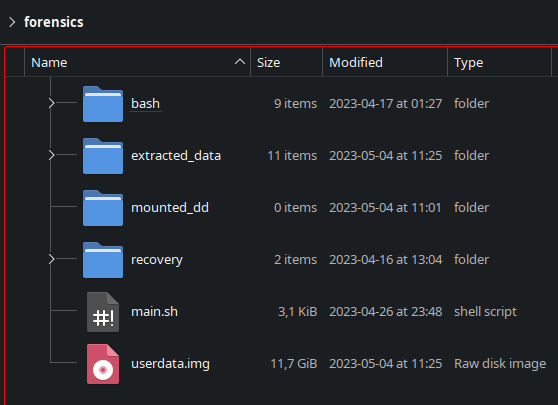
\includegraphics[width=0.85\textwidth]{main_dir.png}
    \caption{Darbo katalogo struktūra}
    \label{fig:workdir}
\end{figure}

\newpage Katalogas „bash“ talpina visus reikiamus skriptus. Katalogas „mounted\textunderscore dd“ yra skirtas „userdata“ atvaizdui užmontuoti. Katalogas „recovery“ saugo savyje du atstatymo režimo atvaizdus - vienas originalus išgautas iš „Samsung“ .tar.md5 originalios programinės įrangos atvaizdo, bei antras neoficialus „TWRP“ atvaizdas. Darbo kataloge taip pat talpinamas „main.sh“ failas bei „userdata.img“ ištrauktas atvaizdo failas. „extracted\textunderscore data“ kataloge talpinami visi išgauti bei išanalizuoti failai (5 pav.): 

\begin{figure} [h]
    \centering
    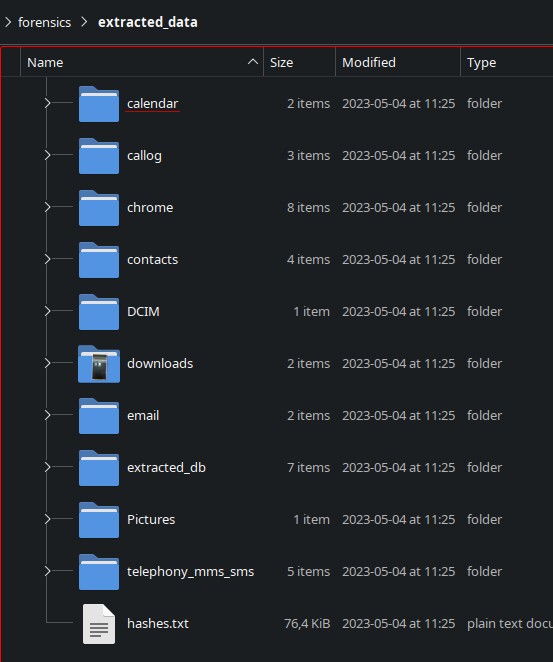
\includegraphics[width=0.80\textwidth]{extraction_dir.png}
    \caption{Ištrauktų duomenų katalogo struktūra}
    \label{fig:extractdir}
\end{figure}
Katalogai: calendar, callog, chrome. contacts, email, telephony\textunderscore mms\textunderscore sms saugo duomenų bazes ištrauktas iš userdata.img atvaizdo. Katalogai DCIM, Pictures, Downloads saugo failus, kurie buvo patalpinti įrenginio vidinėje atmintyje. Katalogas extracted\textunderscore db talpina išanalizuotų duomenų bazių rezultatus. Failas hashes.txt talpina SHA-512 maišos kodą visiem failams, kad būtų galima lengvai palyginti ar failai nebuvo modifikuoti tarp jų išgavimo ir perkėlimo į kitą kompiuterį.

Visi reikalingi analizei failai yra sukaupti šiame kataloge, ir šį katalogą reikėtu pateikti teismui kaip įrodymus.
\clearpage

\subsection{Išanalizuotų .db failų apžvalga}
Šiame poskyryje matomos iliustracijos, rodo tyrimo metu išgautus iš „Samsung Galaxy S3 NEO“ įrenginio duomenis.  Visi šie duomenys buvo sukurti ir parengti šiam darbui  - žinutes, skambučiai, kontaktai, kalendoriaus įrašai bei naršyklės duomenys  buvo specialiai parengti šiam tyrimui. Visi vardai, telefono numeriai bei žinučių turinys yra fiktyvus.\\

6 pav. matome dalį išanalizuoto messages.txt failo. Faile duomenys grupuojami pagal telefono numerius ir surašomi pagal datą.
\begin{figure} [h]
    \centering
    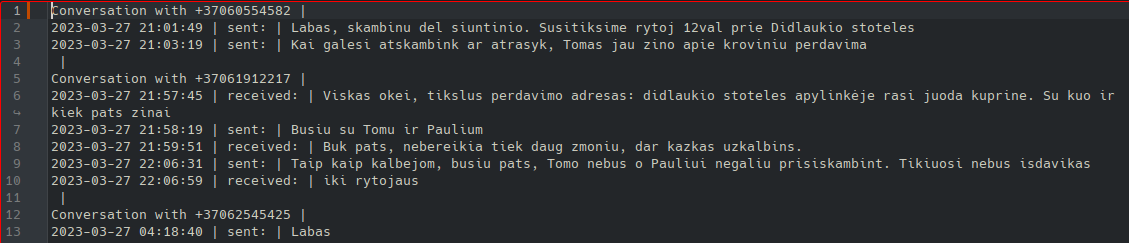
\includegraphics[width=0.85\textwidth]{pav_sms.png}
    \caption{Žinučių .txt failas}
    \label{fig:messages}
\end{figure}


7 pav. matome dalį išanalizuoto login\textunderscore data.txt failo. Matome prisijungimo URL adresą, prisijungimo vartotojo vardą bei slaptažodį.

\begin{figure} [h]
    \centering
    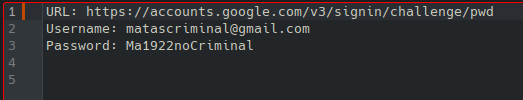
\includegraphics[width=0.85\textwidth]{login-example.png}
    \caption{Prisijungimo duomenų .txt failas}
    \label{fig:login}
\end{figure}
8 pav. matome dalį išanalizuoto cookies\textunderscore data.txt failo. Matome slapukų kilmę, bei jų vertes.

\begin{figure} [h]
    \centering
    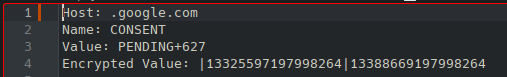
\includegraphics[width=0.85\textwidth]{cookies-example.png}
    \caption{Cookies slapukų .txt failas}
    \label{fig:cookies}
\end{figure}
9 pav. matome dalį išanalizuoto browsing\textunderscore history.txt failo. Matome puslapio pavadinimą, URL adresą bei jo atidarymo datą ir valandą.

\begin{figure} [H]
    \centering
    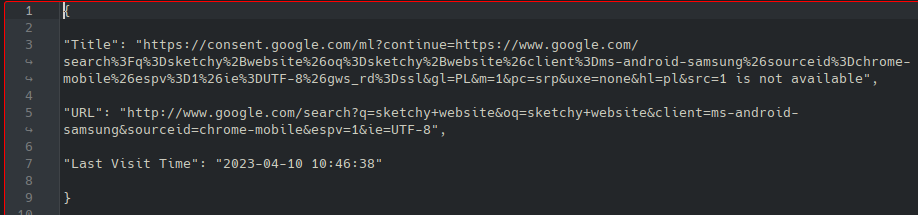
\includegraphics[width=0.85\textwidth]{browsing_history.png}
    \caption{Naršyklės istorijos .txt failas}
    \label{fig:history}
\end{figure}


\newpage
10 pav. matome dalį išanalizuoto call\textunderscore logs.txt failo. Matome skambučio datą, telefono numerį, skambučio trukmę sekundėmis bei tipą: 1- išeinantis skambutis, 2 - įeinantis skambutis.
\begin{figure} [H]
    \centering
    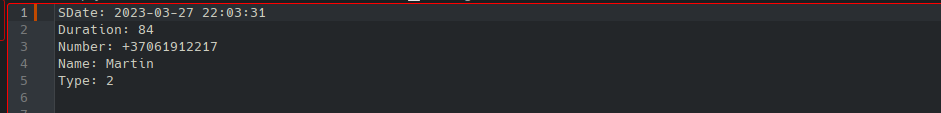
\includegraphics[width=0.85\textwidth]{callog.png}
    
    \caption{Skambučių istorijos .txt failas}
    \label{fig:callog}
\end{figure}

11 pav. matome dalį išanalizuoto contacts.txt failo. Matome užrašytus adresų knygelėje kontaktus su jų pavadinimais bei telefono numeriais.
\begin{figure} [H]
    \centering
    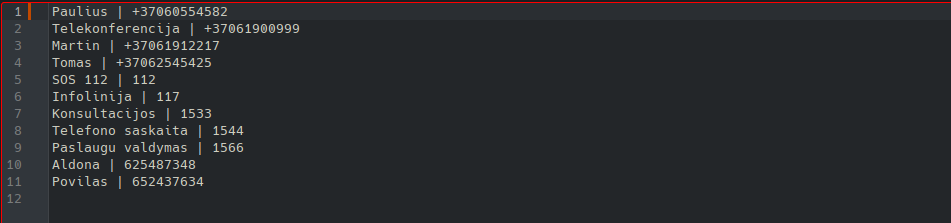
\includegraphics[width=0.85\textwidth]{contacts.png}
    
    \caption{Kontaktų .txt failas}
    \label{fig:contacts}
\end{figure}

12 pav. matome dalį išanalizuoto calendar.txt failo. Matome užrašytą įvykį su jo data, pavadinimu, bei komentarais.
\begin{figure} [H]
    \centering
    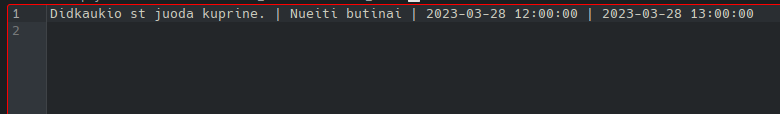
\includegraphics[width=0.85\textwidth]{calendar.png}
    
    \caption{Kalendoriaus.txt failas}
    \label{fig:calendar}
\end{figure}

Visi failai yra talpinami viename kataloge, bei yra užrašyti .txt formatu, kad būtų galima juos atidaryti ir peržiūrėti kiekvienoje operacinėje sistemoje. Šie failai yra itin svarbūs analizei, nes juose galime rasti daug vertingos informacijos. Dėl to kad su testuojamu įrenginiu nukeliavau į kitą valstybe, galime gauti konkrečia datą ir valandą kada buvo peržengta valstybės sieną (13 pav.):
\begin{figure} [H]
    \centering
    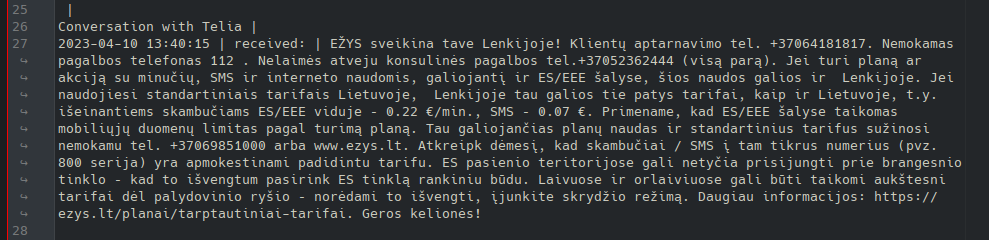
\includegraphics[width=0.85\linewidth]{sms_country.png}
    \caption{SMS žinutė nuo tinklo operatoriaus apie valstybės sienos peržengimą}
    \label{fig:country-borders}
\end{figure}
 %Conclusions section
\sectionWithoutNumber{\keyWordConclusions}{conclu}

Sukurtas įrankis, turi daug funkcionalumų. Gali automatiškai arba rankiniu būdu išgauti duomenis iš daugelio mobiliųjų įrenginių.  Įrankis tinkamas telefonams su ekrano užraktu bei be ekrano užrakto. Įrankis gali ištraukti duomenis iš „Android“ įrenginio „userdata“ particijos atvaizdo, bei gauti juos iš įrenginio, kuris jau paleistas „TWRP“ režime.  Darbo eigoje sukurtas įrankis gali taip pat ištraukti ir apdoroti SMS, kontaktų, skambučių, bei naršyklės duomenų bazes. Taip apdorota medžiaga gali būti panaudota teisminei ekspertizei. Skriptas turi daug informacinių dialogų, kurie leidžia vartotojui lengvai suprasti kas vyksta ir kokius žingsnius reikia įvykdyti, kad duomenų išgavimas vyktų sklandžiai.

Įrankis veikia su daugeliu Samsung įrenginių, bei su kitais įrenginiais, kuriems turime galimybę suteikti „root“ teises arba įrašyti neoficialų atstatymo režimą. 

Darbo metu atliktame tyrime panaudotas įrankis sėkmingai ištraukia duomenis iš „Samsung Galaxy S5“ (veikiančio su naujausia jam prieinama „Android 6.0.1“ versiją) bei  „Samsung Galaxy S3 NEO“ (veikiančiu su naujausia jam prieinama „Android 4.4.4“ versiją). Iš šių mobiliūjų įrenginių pavyko išgauti visus analizei vertingus failus, o prireikus, tolimesnei analizei, įrankis suteikia galimybę sumontuoti atvaizdą ir atlikti analizę rankiniu būdu, analizuojant kitų programėlių duomenų bazes. 

Įrankis ne tik išgauna duomenis, bet ir juos tinkamai suformatuoja, į lengvai skaitomus tekstinius failus. Šis funkcionalumas leidžia žmonėms kurie niekada nedirbo su duomenų bazių analize lengvai peržiūrėti duomenis, tokius kaip SMS žinutes sudėliotas chronologiškai pagal gavėją, naršomų internetinių puslapių istoriją su naršymo datomis, bei URL adresais. 

Kadangi tai tik pirma pabaigta įrankio versija, jo automatinė duomenų išgavimo procedūra ribota veikti su Samsung įrenginiais. Atsižvelgiant į tai jog Lietuvoje pirmauja Samsung gamybos įrenginiai, sukurtas įrankis gali būti vertingas teisminėms analizėms. Remiantis Statcounter statistika \cite{StatcounterLithuania} (14 pav.),  virš trečdalis Lietuvoje naudojamų įrenginių yra Samsung gamybos.
\begin{figure} [h]
    \centering
    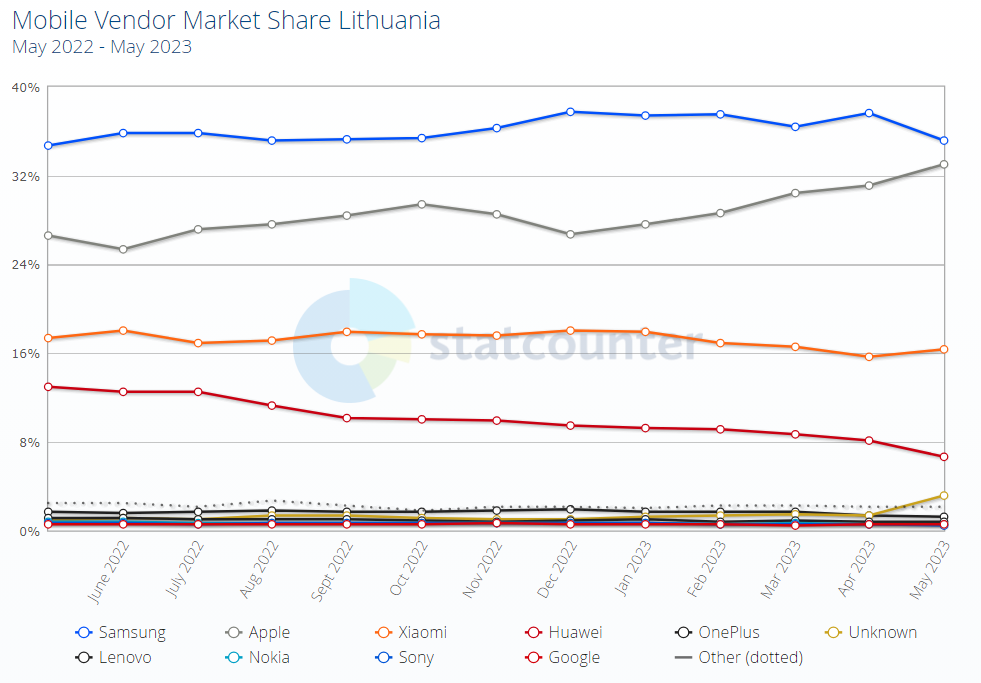
\includegraphics[width=0.85\linewidth]{stat_lt2.png}
    \caption{Mobiliųjų įrenginių pasiskirstymas pagal gamintojus Lietuvoje}
    \label{fig:LT_tel_statistics}
\end{figure}

%ateities darbų gairės, planas/next steps of the work
\sectionWithoutNumber{Ateities tyrimų planas}{future}{Ateityje būtų vertinga tiksliau išanalizuoti įrenginius su „force-encrypt“ šifravimu įjungtu pagal gamintojo numatymus. Dauguma mobiliųjų įrenginių naudoja „fastboot“ paleidimo įkroviklį, kurį būtina atrakinti, kad būtų galimybė suteikti root teises arba įrašyti „TWRP“ atstatymo režimą. Be aukštesnių root teisių, duomenų particijos atvaizdo išgavimas nėra įmanomas. 

Reikėtu taip pat atsižvelgti į SQL užklausas, nes kai kurios iš jų ar failo keliai yra betarpiškai parengti veikti su „Samsung“ mobiliais įrenginiais. Ši modifikacija nereikalauja daugelio pakeitimų kode, tad nebūtų sunku sukurti dar viena pasirinkimų menu, duomenų bazių analizės skripte, kuriame galėtume nurodyti įrenginio gamintoja, ir atitinkamai pagal tai apdoroti failus atitinkamuose aplankuose bei su atitinkamomis užklausomis

Jeigu betarpiška analizė būtų teisėta,  įranki būtų galima patobulinti papildomu funkcionalumu, kuris leistų apdoroti įrenginius be microSD kortelių skaitytuvo. Būtų galima sukurti skriptą kuris betarpiškai ištrauktų reikiamus analizei failus, praleidus atvaizdo kūrimą.

Galiausiai, būtų galima tyrinėti dar kelis atvejus, pavyzdžiui kiniškus įrenginius, nes jų saugumo lygis yra žymiai žemesnis nei kitų. Kai kurie „Xiaomi“ gamintojo įrenginiai, priklausomai nuo programinės įrangos versijos, buvo parduodami su galimybe įjungti „root“ teises betarpiškai „Kūrėjo parinkčių“ menu, nereikalaujant jokių modifikacijų įrenginio particijose ar įkroviklyje. Šią parinktį matome šioje iliustracijoje (15 pav.):
\begin{figure} [h]
    \centering
    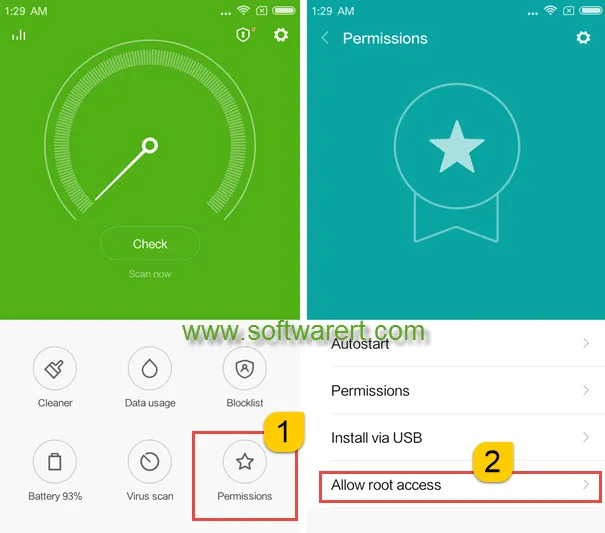
\includegraphics[width=0.80\linewidth]{xiaomi_root.png}
    \caption{„Xiaomi“ įrenginių nustatymas leidžiantis įjungti root teises}
    \label{fig:xiaomi-root}
\end{figure}

Toks skriptas taip pat suveiktų su visais įrenginiais kuriems vietoj įrašinėti neoficialų atstatymo režimą, suteiksime „root“ teises sistemos lygyje.}


 %file literatureSources.bib
\referenceSources{literatureSources}

\end{document}
